\documentclass{article}

\usepackage[margin=1in]{geometry}
\usepackage{amsmath,graphicx}
\usepackage{color}
\usepackage{hhline}
\usepackage{natbib}
\usepackage{aas_macros}

\newcommand{\expon}[1]{e^{#1}}
\newcommand{\e}[1]{\times 10^{#1}}
\newcommand{\tableend}{\\}

\title{A Wideband Self-Consistent Disk-Averaged Spectrum of Jupiter Near 30 GHz and Its Implications for NH$_{3}$ Saturation in the Upper Troposphere}
\date{\today}
\author{Ramsey Karim, David DeBoer, Imke de Pater, Garrett Keating}

\begin{document}

\maketitle
\abstract{
	We present a new set of CARMA measurements of Jupiter's microwave thermal emission near the 1.3 cm ammonia (NH$_{3}$) absorption band, which we use to investigate ammonia abundance in the upper troposphere, near $0.3<P<2$ bar, based on radiative transfer modeling.
	We find ammonia to be present at about half the nominal value below the $P\sim 0.8$ bar NH$_{3}$ cloud layer specified in \citealt{2016Sci...352.1198D}, corresponding to a new deep ($P \sim 8$ bar) atmosphere fractional abundance of $2.4\e{-4}$.
	This conclusion is not extended past $P = 8$ bar, since our measurements have no sensitivity at this depth and the result would contradict Galileo probe results.
	We find the NH$_{3}$ cloud-forming region between $0.3 < P < 0.8$ bar to be globally subsaturated by 55\% on average, in accordance with the result in Gibson et al. 2005.
	While these data are not very sensitive to the region above the cloud layer, we are able to set an upper limit of $2.4\e{-7}$ on the abundance here, although both our fitting process and the Clausius-Clapeyron equation of state suggest something closer to $\sim 2\e{-8}$.
	All three results agree that NH$_{3}$ abundance is a factor of 2 lower than suggested by Galileo probe results above $P < 2$ bar, a conclusion consistent with the Gibson et al. 2005 result as well as the ground-based radio models discussed in de Pater et al. 2001.
}

NEED TO REFER TO THE TABLES AND FIGURES IN THE TEXT

\section{Introduction} \label{s:introduction}
	Microwave observations of Jupiter's atmosphere are generally dominated by pressure-broadened spectral features of ammonia gas in the troposphere.
	The most notable feature in this region of the gas giant's thermal spectrum is the 1.3 cm NH$_{3}$ inversion/absorption band, first reported as a single, broad line by \citealt{1968ApJ...154.1077L} and found by \citealt{1978Icar...35...44K} to be a ``diagnostic of the pressure and temperature profiles in the cloud-forming region of the Jovian atmosphere.''
	As we continue to sample Jupiter's thermal spectrum around this band, we can better characterize the shape of this spectral feature, which, through proper analysis, provides us with a deeper understanding of the planet's vertical structure and improves Jupiter's usefulness as a radio calibrator.

	Decades of disk-averaged, and more recently, spatially resolved, observations as well as in situ probe measurements have contributed to our understanding of the planet's atmospheric structure,
%Ammonia's presence in the jovian atmosphere was first noted by \citealt{1937ApJ....86..321W} using evidence from the visible spectrum, but it was not until the 1950s-60s that the radio spectrum was explored more thoroughly in order to derive a consistent ammonia abundance.
%This mid-to-late 20th century investigation of Jupiter's microwave spectrum suggested 
	initially revealing a relatively straightforward model involving an adiabatic atmosphere with roughly solar NH$_{3}$ abundance in the deep atmosphere, which is considered to be well-mixed.
	The detailed radiative transfer analysis presented in \citealt{1985Icar...62..143D} agrees, stating solar NH$_{3}$ abundance to within a factor of 2 until $P < 0.5$ bar, above which NH$_{3}$ drops by $\sim 10^{3}$.
	This depletion is consistent with NH$_{3}$ condensation following the saturated vapor curve.

	Modern efforts to uncover more about the planet's vertical structure have also raised new questions \citep{2005Icar..173..425D}.
	The Galileo probe mission of the 1990s presented {\sl in situ} measurements of NH$_{3}$ abundance that arguably conflict with models derived from ground-based observations, creating what was described in that paper as the ``Galileo's Ground-based Microwave Paradox.''
	Probe measurements suggest that NH$_{3}$ abundance should be nearly 4$\times$ solar
		\footnote{We designate a solar model based on the most recent proto-solar elemental abundance estimates (\citealt{2009ARA&A..47..481A}). N/H2 is taken to be $1.48 \e{-4}$. Henceforth, the solar NH$_{3}$ abundance value is $1.28 \e{-4}$.}. 
	Given the previously accepted model, this result was jarring to our understanding of the atmosphere's structure and dynamics.  To improve this understanding additional datasets are needed along with updated modeling using the latest measurement microwave properties of, primarily, ammonia gas.

	This work presents new ground-based observations over a very wide bandwidth with an interferometer that does not resolve the planet so that more accurate disk-averaged brightness temperatures may be determined.  It also provides a single systematically-consistent dataset over its band (27-35 GHz) that may be used in conjunction with the many decades of observations of our largest planet ({\em e.g.} \citealt{1978Icar...35...44K}, \citealt{2003ApJS..148...39P}, \citealt{2011ApJS..192...19W}, \citealt{2005Icar..173..439G}, \citealt{2016Sci...352.1198D}).
	Having a well-calibrated systematically-consistent dataset over this broad bandwidth complements the single absolutely calibrated point at near 28.5 GHz in \citealt{2005Icar..173..439G} (hereafter JG).
	 JG corrects and discusses all three of these sets, concluding that NH$_{3}$ is globally subsolar between $0.6 < P < 2$ bar and subsaturated by more than 50\% between $0.4 < P < 0.6$ bar.
	 
	Based on these measurements we fine-tune the model presented in \citealt{2001Icar..149...66D} and extended in \citealt{2016Sci...352.1198D} which based on Galileo measurements takes NH$_{3}$ abundance to be $4.5 \times$ solar ($5.72 \e{-4}$) in the deep atmosphere and then follows the saturated vapor curve within and above the cloud layers.
	This model, described in more detail in Section \ref{s:model}, is henceforth referred to as the ``nominal'' model and serves as the base model for this work.
	%From this point, our radiative transfer analysis of the available measurements, described below, should tune this nominal model into a Radio Model of improved accuracy.


\section{Data} \label{s:data}
	One of the last studies conducted with the Combined Array for Research in Millimeter-wave Astronomy (CARMA) was a CO power spectrum survey which aimed to measure the CO(1-0) transition in redshift $\sim 3$ galaxies (\citealt{2015ApJ...814..140K}; \citealt{2016ApJ...830...34K}, hereafter referred to as COPSS).
	The compact, 8-element Sunyaev-Zel'dovich Array (SZA) subset of CARMA was used to take various field scans between 27-35 GHz to measure the redshifted $\lambda_{0} = 115$ GHz line.
	COPSS used Mars as the primary calibrator, and Jupiter as the secondary calibrator scans of Jupiter.
	It is these Jupiter observations, taken between December 2014 and the array's decommissioning in April 2015, that are used in this work.

	The SZA is a set of eight 3.5 m elements sensitive to left circularly polarized radiation in a compact array (\citealt{2015ApJ...814..140K}).
	Since it does not resolve the planet, the array is well-suited for accurate measurements of Jupiter's total flux density.
	The calibration data from COPSS comprise flux densities spanning 15 channels from 27-35 GHz (0.8 to 1.1 cm) and 100 days between December 2014 and April 2015.
	Error estimates accompanying the data have typical values of $\sim0.01$ Jy and account only for thermal error.
	Uncertainty in the absolute flux calibration is preliminarily estimated at $<5\%$ according to COPSS, but we present our own thorough investigation in Section \ref{s:error}.
	CARMA in its entirety is a fairly spectrally stable instrument, so we expect relative uncertainty to be somewhat smaller than absolute uncertainty (sec. \ref{s:xxx}).

\subsection{Flux Measurement Reduction} \label{}
	Reduction of these data converts a time series of flux densities to a single brightness temperature on channel-by-channel basis.
	The process also isolates and corrects for a variety of systematics throughout the process.
	The result is 15 time- and disk-averaged measurements of Jupiter's brightness near the 1.3 cm ammonia absorption band.

	The effects of Jupiter's distance from Earth during the observational period are removed through distance normalization to the nominal value of 4.04 AU, ``flattening'' each channel's measurement as is made evident between the two panels in Figure \ref{fig:raw}.
	This step facilitates examination of antenna gain error, indicated by the variance in the normalized points as well as the cross-channel behavior during individual observations.
	\begin{figure}
		\centering
		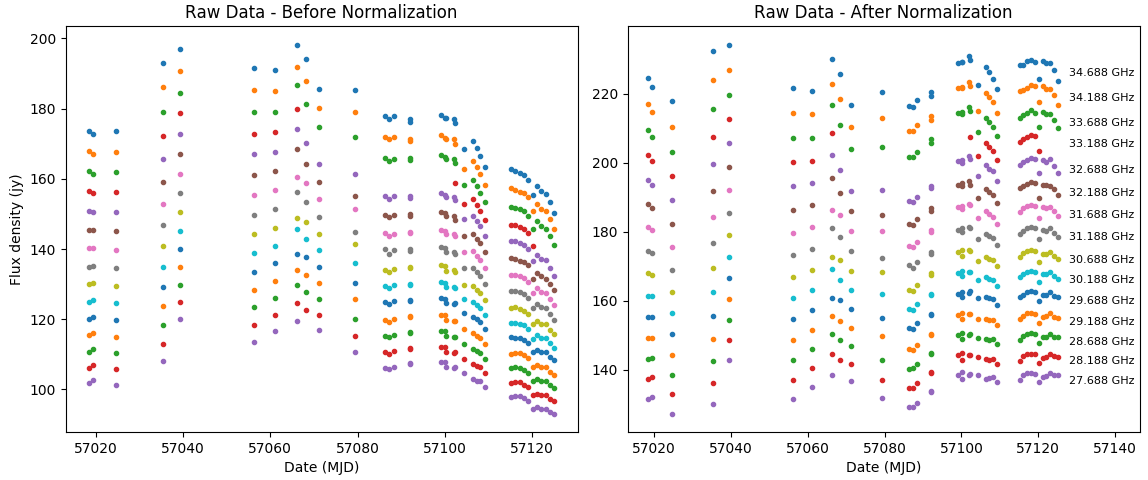
\includegraphics[width=\textwidth]{final_raw.png}
		\caption{\label{fig:raw}Flux density measurements by time, before and after distance adjustment.}
	\end{figure}
	Jackknife testing, discussed in more detail in Section \ref{s:jackknife}, reveals an additional artifact at this stage.
	The series of flux densities for each channel show positive linear correlation with Jupiter's elevation in the sky at the time of observation, indicating some potential issue with airmass calibration in the original measurements.
	\begin{figure}
		\centering
		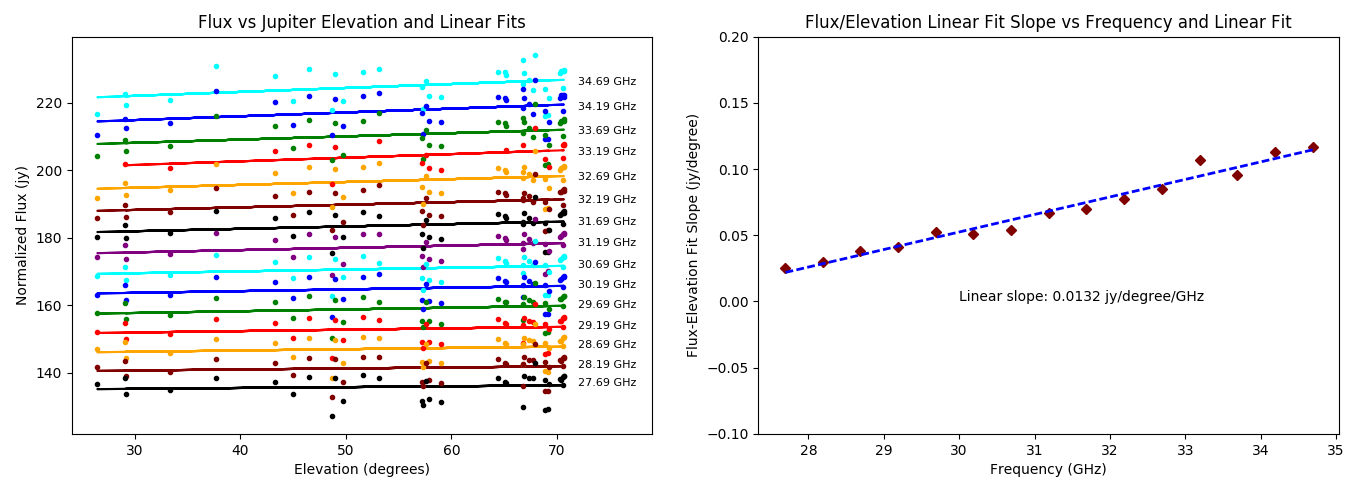
\includegraphics[width=\textwidth]{final_airmass.png}
		\caption{\label{fig:air}Indication of linear dependence of flux on elevation, and more importantly, linear dependence of flux-elevation slope on frequency.}
	\end{figure}
	The slopes of each channel's correlation are positive linear by frequency and therefore simple to normalize out, as demonstrated in Figure \ref{fig:air}, assuming that the measurements taken at higher elevations through thinner layers of atmosphere are more accurate.

	% Averaging
	The flux densities are averaged across time with weights corresponding inversely to the thermal error on each measurement.
	Averages are calculated as
	$$F_{\nu,\,meas} = \langle F_{\nu} \rangle = \frac{ \sum_{i} w_{\nu, i} F_{\nu,i} }{ \sum_{i} w_{\nu, i} }$$
	where $$w_{\nu, i} = 1/\sigma_{\nu, i}^{2}$$
	such that $\sigma_{\nu, i}$ is the stated thermal error in janskys on the $i$th measurement for a given channel.
	Averaging the flux densities themselves is fairly straightforward; the rest of this section will discuss the application
	of meaningful error estimates.

\subsubsection{Absolute ($\sigma_{A}$) and Relative ($\sigma_{R}$) Uncertainty} \label{s:error}
	We define two distinct error measurements for the data set: absolute uncertainty $\sigma_{A}$ and relative uncertainty $\sigma_{R}$.
	Absolute uncertainty quantifies our estimate of the overall calibration accuracy of the SZA, estimating how close the data are to the actual values.  It is determined by the systematics of the instrument.
	%The $\sigma_{A}$ measurement cannot wildly upset the relationship between points within this set; it is primarily a characteristic of the ensemble as a whole.
	From COPSS, an estimated upper limit of $<5\%$ on this calibration error is quoted.

	Relative uncertainty quantifies the stability of each channel with respect to the others, estimating internal consistency rather than absolute accuracy.
	CARMA has strong spectral stability and can observe this feature in the strongly correlated cross-channel behavior displayed in Figures \ref{fig:raw} and \ref{fig:air}, which suggests that the $\sigma_{R}$ measurement, while allowing some independent uncertainty on points, is expected to be smaller than $\sigma_{A}$ and so will not have as great an effect on the overall position of the ensemble.
	$\sigma_{R}$ is useful in defending the use of the relative structure of the ensemble as a comparably reliable tool to the absolute position as well as quantifying a model's match to this relative structure during the model-comparison process.
	$\sigma_{A}$, by contrast, serves as a more conventional uncertainty estimate.

	We approach the absolute uncertainty $\sigma_{A}$ estimate using statistical properties of the flux density ensemble along with their stated thermal errors.  The absolute uncertainty is the quadrature  sum of the weighted average of the individual data and the thermal noise of each measurement and may be written
	$$\sigma_{A}(\hat{\sigma}, \hat{n}) = \hat{\sigma}^{2} + \hat{n}^{2}$$
The first term is 
		$$\hat{\sigma}^{2} = \frac{\sum_{i} w_{i} \big( F_{\nu,i} - \langle F_{\nu} \rangle \big)^{2} }{\sum_{i} w_{i}}$$
	The second term, the thermal contribution $\hat{n}$, is calculated as the reciprocal sum of thermal uncertainties for a given channel.
	With $w_{i}$ defined above, $\hat{n}$ is
	$$ \frac{1}{\hat{n}^{2}} = \sum_{i} w_{i} $$
	In this way, we merge statistical 1-sigma error on a channel's flux ensemble with the thermal uncertainty of the points themselves and produce the value $\sigma_{A}$, our estimate of uncertainty on the absolute calibration of the instrument.
	This we find to be closer to $\sim2\%$, which falls under the upper limit stated by COPSS.

	Relative uncertainty $\sigma_{R}$ comprises both thermal contribution as well as the tendency of each channel to deviate from the others.
	A perfectly stable instrument should exhibit a consistent cross-channel response to small, day-to-day variation in observed flux; unexpected behavior should be reflected in $\sigma_{R}$.
	We compare observations across channels by normalizing each channel with its average.\footnote{Until now, all averages have been across time, isolated to each channel.
	In this section, that will no longer be the case, so averages will be marked as either channel averages ($\nu$) summed across all observations as before, or ``daily'' averages ($i$) calculated with sums across all channels, isolated to each observation.}
	The normalized measurements are denoted $f_{\nu, i}$.
	$$ f_{\nu, i} = \frac{F_{\nu, i}}{\langle F_{\nu, i} \rangle_{\nu}} $$
	This fraction is averaged across each observation to find the daily mean deviation from each channel's respective average.
	A stable instrument's channels would exhibit minimal spread around this daily mean deviation, and any spread should be uncorrelated with channel.
	We isolate the residuals $\delta_{\nu, i}$ from this daily average by subtracting the daily mean deviation from each observation set of normalized measurements, so as to exclude the daily deviation itself and examine each channel's deviation from this deviation.
	These residuals are defractionalized by multiplying by the channel average.
	$$ \delta_{\nu, i} = (f_{\nu, i} - \langle f_{\nu, i} \rangle_{i}) \cdot \langle F_{\nu, i} \rangle_{\nu} $$
	Each channel's behavior is now quantified by its mean deviation from the daily average as well as the spread of these deviations, given by their variance across each channel.
	During this examination, it was noted that the channels had a tendency to vary together in time; they often would pivot around the 31.188 GHz measurement, which remained stable to within $0.5$\% of the measurement value.
	The frequencies at either extreme (27.688 GHz and 34.688 GHz) varied by no more than 6\%.
	It is unclear what causes this linear variation, but it is worth mentioning that even though this estimate describes the uncertainty of these points relative to each other, it is an overestimate.
	There remains some unidentifiable cross-channel dependency.

	We introduce a thermal component as well, calculated by fractionalizing each thermal error by its accompanying measurement, averaging across each channel, and denormalizing with the channel average.
	$$\sigma_{th} = \Bigg\langle \frac{\sigma_{i}}{F_{\nu,i}} \Bigg\rangle_{\nu} \langle F_{\nu, i} \rangle_{\nu} $$

	The final relative uncertainty measurement contains the thermal component $\sigma_{th}$ as well as the mean $\langle \delta_{\nu, i} \rangle_{\nu}$ and standard deviation $\Big\langle (\delta_{\nu, i} - \langle \delta_{\nu, i} \rangle_{\nu})^{2} \Big\rangle_{\nu}^{1/2}$ of the daily deviations by channel.
	The third term, the variance of the channel's daily deviations, dominates the entire measurement and gives each channel a relative uncertainty on the order of a jansky.
	$$ \sigma_{R}^{2} = \sigma_{th}^{2} + \langle \delta_{\nu, i} \rangle_{\nu}^{2}
		 + \Big\langle (\delta_{\nu, i} - \langle \delta_{\nu, i} \rangle_{\nu})^{2} \Big\rangle_{\nu} $$


\subsubsection{Synchrotron Correction}

	The relatively large SZA beam ($\theta_{B} \approx 11'$ full width at half max) contains flux from both thermal and non-thermal components.
	In this frequency regime, synchrotron radiation dominates the non-thermal emission.
	Since we are interested only in the thermal component, we must subtract out the synchrotron radiation from the total observed flux density.

	Jupiter's dynamic synchrotron spectrum has been a subject of discussion since the 1970s when a series of observations suggested time variability in the low-frequency\footnote{\citealt{1976JGR....81.3380K} uses 11-13 cm and 21 cm, considerably longer wavelengths than our 1 cm.} spectrum (\citealt{1976JGR....81.3380K}).
	A survey of that spectrum from 74 MHz up to 8 GHz, described in \citealt{2003Icar..163..434D}, suggests that synchrotron contribution to the planet's radio spectrum drops off above 2 GHz, so we believe that, with frequencies around 30 GHz, our measurements contain negligible synchrotron-induced variability.
	Additionally, \citealt{1976JGR....81.3380K} observes that fluctuations on the order of days did not exceed 10\%, and explores several-year variability with 1-3 month averages, implying that our 5-month average should capture an approximately constant period of synchrotron variability.
	Under this assumption, we use a simplified and time-independent model of synchrotron contribution to recover the thermal spectrum.
	The correction is purely arithmetic and thus does not propagate into uncertainties.

	JG uses a value of 1.5 Jy for the synchrotron contribution to a 28.5 GHz measurement of the thermal spectrum, which has a value of about 145 Jy, based on work done by \citealt{2003Icar..163..449D}.
	In order to adjust extant data in the same frequency regime, JG adopts a relationship of $F_{\nu,\,synch} \sim \nu^{-0.4}$, leading to the local model
	$$F_{\nu,\,synch} =  (1.5 \ Jy)\Bigg(\frac{\nu}{28.5 \ GHz}\Bigg)^{-0.4}$$
	which we apply across our small frequency domain.

	The synchrotron model is subtracted from the time-averaged flux density at each channel, yielding thermal-only flux density measurements:
	$$F_{\nu,\,thermal} = F_{\nu,\,meas} - F_{\nu,\,synch}$$


\subsection{Conversion to Brightness Temperature and Cosmic Microwave Background (CMB) Adjustment} % Neptune 2014 Imke
	
	Thermal radiation flux density $F_{\nu\,thermal}$ is converted to brightness temperature $T_b$ via the Planck function.
	The resulting $T_{b,\,meas}$ from a direct conversion is not yet indicative of the true temperature of the emitter -- it is the contrast between the emitter and the microwave background.
	Correction for this is made during conversion, following a similar adjustment made in \citealt{2014Icar..237..211D}.
	Observed thermal flux density is set equal to a combination of thermal brightness temperature and CMB contribution by the Planck function, as below, allowing $T_{cmb} = 2.725$ K.
	$$ F_{\nu} = \frac{2h\nu^3}{c^2}\Bigg( \frac{1}{\expon{\frac{h\nu}{kT_b}} - 1} - \frac{1}{\expon{\frac{h\nu}{kT_{cmb}}} - 1} \Bigg)
		\frac{\pi R_{eq} R_{p}'}{D^2} $$
	where apparent polar radius is given by $R_{p}' = \sqrt{R_{eq}^{2}\sin^{2}{\phi} + R_{p}^{2}\cos^{2}{\phi}}$.
	Subearth latitude used here is $\phi = 0.15^{\circ}$, which is the average over a tight cluster of
	small, similar $\phi$ values over the four month observation interval according to the JPL Horizons interface.

	Working values at each major step as well as final measurements and associated errors are laid out in Table \ref{tab:1}.
	The $T_b$ values, along with some combination of the $\sigma_{A}$ and $\sigma_{R}$ errors, are appropriate for reproduction in future work.


	% TABLE !!
	\begin{table}
	\centering
	\begin{tabular}{cc || c | c | c | c | c }
	$f$ (GHz) & $\lambda$ (cm) & $F_{\nu,\,meas}$ (jy) & $F_{\nu,\,thermal}$ (jy) & $T_b$ (K) & $\sigma_{A}$ (K) & $\sigma_{R}$ (K) \\\hhline{==#=|=|=|=|=}
	34.688 & 0.864 & 226.612 & 225.225 & 151.013 & 3.180 & 1.359 \tableend
	34.188 & 0.877 & 219.250 & 217.855 & 150.385 & 3.143 & 1.186 \tableend
	33.688 & 0.890 & 211.832 & 210.429 & 149.615 & 3.222 & 1.037 \tableend
	33.188 & 0.903 & 206.006 & 204.594 & 149.876 & 2.531 & 1.244 \tableend
	32.688 & 0.917 & 198.089 & 196.669 & 148.534 & 3.244 & 0.620 \tableend
	32.188 & 0.931 & 191.047 & 189.618 & 147.707 & 3.228 & 0.510 \tableend
	31.688 & 0.946 & 184.615 & 183.177 & 147.235 & 3.240 & 0.316 \tableend
	31.188 & 0.961 & 178.155 & 176.708 & 146.635 & 3.293 & 0.146 \tableend
	30.688 & 0.977 & 171.458 & 170.002 & 145.720 & 3.266 & 0.378 \tableend
	30.188 & 0.993 & 165.546 & 164.080 & 145.347 & 3.382 & 0.395 \tableend
	29.688 & 1.010 & 159.553 & 158.077 & 144.794 & 3.515 & 0.675 \tableend
	29.188 & 1.027 & 153.335 & 151.849 & 143.911 & 3.584 & 0.769 \tableend
	28.688 & 1.045 & 147.477 & 145.981 & 143.225 & 3.679 & 0.960 \tableend
	28.188 & 1.064 & 141.586 & 140.080 & 142.369 & 3.767 & 1.147 \tableend
	27.688 & 1.083 & 136.081 & 134.563 & 141.757 & 3.875 & 1.368 \tableend
	\end{tabular}
	\caption{\label{tab:1}Values at each frequency through major correction steps, after averaging. $F_{\nu,\,meas}$ and $F_{\nu,\,thermal}$ are normalized to 4.04 AU. $T_b$ values include CMB correction. Error estimates are given for the final $T_b$ values only.}
	\end{table}


\subsection{Jackknife Testing} \label{s:jackknife}
In order to investigate whether identifiable systematics are present, we conducted a set of jackknife tests during which we run arbitrarily selected halves of the time-series data through the analysis pipeline and observe the average resulting change in brightness temperatures.
	The data are halved both on meaningless criteria, such as odd/even index, as well as by criteria with more systematic potential, such as Jupiter's horizontal elevation at the time of observation.

	It was mentioned earlier that what may be an airmass calibration error in the raw data was detected by one of these jackknife tests, specifically one using Jupiter's elevation.
	After this correction, all subsequent jackknife tests amount to nothing more than noise at less than 2\% variation from the full-range values, indicating that we have identified all major systematics about which we have information.
	The consistency of our measurements with the Gibson and WMAP points corroborates this, or at least suggests that we all suffer from the same unknown systematics.


\section{Model Fitting} \label{s:model}

	As briefly discussed in Section \ref{s:introduction}, the main source of radio opacity in Jupiter's atmosphere is ammonia gas.
	The following subsections outline our methods for determining NH$_{3}$ abundance in the part of the atmosphere to which our measurements are sensitive.

\subsection{Nominal NH$_{3}$ Profile}

	Our calculations use the radiative transfer code most recently used in \citealt{2016Sci...352.1198D}; this code is based upon an atmosphere in thermochemical equilibrium, as described in detail by \citealt{2005Icar..173..425D}.
	As in \citealt{2016Sci...352.1198D}, we assume for our nominal model that all constituents (NH$_{3}$, H$_{2}$S, CH$_{4}$, and H$_{2}$O) are enhanced by a factor of 4.5 above solar in the deep atmosphere ($P > 8$ bar), as observed by the Galileo probe for NH$_{3}$, H$_{2}$S, and CH$_{4}$ (\citealt{1998JGR...10322847F}, \citealt{1999BAAS...31.1154M}, \citealt{1998JGR...10322929S}, \citealt{2004Icar..171..153W}).
	At higher altitudes, NH$_{3}$ will be partially dissolved in the water cloud ($\sim 6$ bar), will form the NH$_{4}$SH cloud ($\sim 2.5$ bar), and at $P < \sim 0.8$ bar will condense into its own ice cloud and follow the saturated vapor curve.
	In our nominal model we thus assume an NH$_{3}$ abundance of $5.72 \e{-4}$ in Jupiter's deep atmosphere, which is diminished at altitudes at which clouds form.
	We adopt a 100\% humidity within and above the NH$_{3}$ ice cloud in our nominal model.
	This results in a constant abundance of $1.20\e{-7}$ near and above tropopause.

\subsection{Model Generation Through Perturbation}

	Starting with the nominal NH3 abundance profile described above, we apply to it small, unity-order adjustments, which in turn gives us the ability to generate a range of theoretical emission profiles.
	These theoretical profiles are compared to the available measurements in order to isolate an abundance profile in maximal agreement with observational evidence.
	The profiles are generated using a radiative transfer software, pyplanet, described in \citealt{2014Icar..237..211D} for its use on Neptune's atmosphere. The software ignores potential opacities from clouds.

	We begin this process by separating the atmosphere into regions of altitude based on their radiative contribution to our measurements, according to the nominal NH$_{3}$ abundance model.
	These contribution functions, shown on the left panel of Figure \ref{fig:tp}, are most prevalent between $0.5 < P < 0.8$ bar.
	This layer coincides with the NH3 ice cloud-forming region, during which NH3 follows the saturated vapor curve, as indicated by the nominal abundance profile shown on the right panel of Figure \ref{fig:tp}.
	We apply to this region, defined by its plummeting NH$_{3}$ abundance, a constant humidity multiplier $RH$.
	Through this parameter, we will tune humidity in the cloud-forming region to fit observations.

	We similarly treat the regions of constant NH$_{3}$ abundance above and below this layer, granting them their own modifying constants.
	The sub-cloud region, defined as the region of approximately constant NH$_{3}$ abundance between the NH$_{3}$ cloud and $P < 8$ bar, is modified by the parameter $\alpha_{d}$.
	As we are not sensitive to anything below $P > 8$ bar, we jump the abundance below this point back to the nominal model, which is motivated by Galileo measurements sensitive to this deeper region.
	The region of constant abundance above tropopause is modified by the parameter $\alpha_{h}$.

	These parameters, $RH$, $\alpha_{d}$, and $\alpha_{h}$, form a three-parameter grid across which we create slightly modified versions of the nominal abundance model.
	Each element of the grid is run through the radiative transfer software to generate a theoretical emission profile, and each of these profiles is compared to the emission measurements such that each point on the three-dimensional grid is associated with a $\chi^{2}$ value.
	We search the parameter space, bound by a physically reasonable range of unity-order constants, for a global minimum. This minimum is explored to within 0.5\% resolution of the nominal value.
	The abundance profile associated with this minimum is taken to be the profile in maximal agreement with observational evidence. Uncertainty for each parameter is approximated as the region in which the local $\chi^{2}$ value is less than $2\times$ the minimum $\chi^{2}$ value.

	\begin{figure}
		\centering
		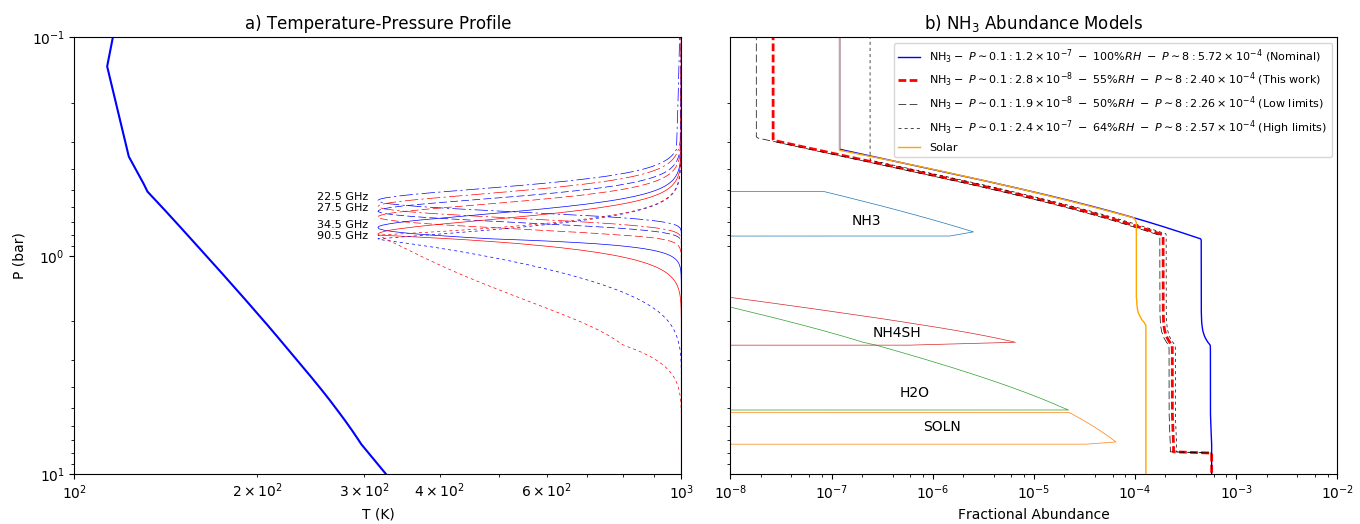
\includegraphics[width=\textwidth]{final_tp_const.png}
		\caption{\label{fig:tp}On the left, the temperature-pressure profile used in our model of Jupiter's atmosphere. Several weighting functions are overlaid on the right edge of this figure. On the right, the fractional NH$_{3}$ abundances according to the solar and nominal constituent abundance models plotted next to three selected models. The red dashed line indicates the abundance model that agrees best with the measurements using our 3-parameter grid fit, and the thinner black lines indicate global high- and low-abundance limits using the error bounds for each parameter. The lower bound for high atmosphere abundance is not certain; this plot uses the small value resulting from the Clausius-Clapeyron equation of state. Cloud levels are overlaid on the left hand side of this panel.}
	\end{figure}


\section{Results} \label{s:results}

	Our 15 SZA measurements of Jupiter's atmospheric thermal emission show a smoothly sloped sample of the shorter-wavelength side of the 1.3 cm NH$_{3}$ absorption band.
	We compare them with the surrounding WMAP and Klein \& Gulkis sets as adjusted in JG as well as Gibson's original point at 28.5 GHz, and updated VLA measurements from \citealt{2016Sci...352.1198D}.
	The SZA observations are consistent to well within 1\% with points from these existing measurements that fall between 27-35 GHz.

	We implement the model-measurement comparison scheme discussed in the previous section and generate a grid of theoretical emission profiles and corresponding $\chi^{2}$ comparison results.

\subsection{Sub-Cloud Abundance $\alpha_{d}$}

	We examine NH$_{3}$ abundance below the cloud-forming region relative to the nominal abundance value of $5.72\e{-4}$.
	The model comparison process indicates a value of $2.40\e{-4}$, with uncertainty bounding it between $[2.26, 2.57] \e{-4}$.
	This value produces a predicted emission profile that agrees well with all observations, especially the high frequency WMAP points most sensitive to the deeper atmosphere.

\subsection{Relative Humidity $RH$}

	Humidity is examined relative to the saturation curve region in the nominal model, roughly between $0.3 < P < 0.8$ bar.
	The nominal model follows 100\% humidity, so our results will be considered relative to a fully saturated model.
	Results of the comparison process suggest a humidity of $56.5\%$, bounded between $[50\%, 63.5\%]$.
	This humidity adjustment produces models that are consistent with all observations, especially the lower frequency CARMA points, the Gibson point that are most sensitive to this pressure range.

	JG states that NH$_{3}$ abundance is, on average, subsaturated by at least a factor of 2 at $P < 0.6$ bar.
	Our results corroborate this subsaturation, within our own pressure regime stated above, down to the factor of 2, but add a tighter bound based on 4 independent sets of measurements.


\subsection{High Atmosphere Abundance $\alpha_{h}$}

	High atmosphere abundance is examined relative to the nominal value of $1.2\e{-7}$.
	The comparison process suggests a value of about $2.8\e{-8}$, nearly one fifth of the original, but yields an upper bound of $2.4\e{-7}$, twice the original value.
	Since we are not very sensitive to these pressures, we are not able to provide a lower bound.

	This result relies primarily on the lowest frequency WMAP measurement but has some input from the lower frequency CARMA measurements.
	It is difficult to place any reasonable bound on the high atmosphere abundance due to the lack of data near the band center; the Klein \& Gulkis measurements were deemed to uncertain for our comparison, but all tend toward temperatures higher than the WMAP point.
	Higher temperature at the band center would indicate a lower pressure departure from the saturation curve and consequently a smaller high atmosphere abundance.
	The precise number found in our analysis is likely meaningless -- nevertheless, it is quite possible that the high atmosphere abundance should be smaller than its value in the nominal model.

	\begin{figure}
		\centering
		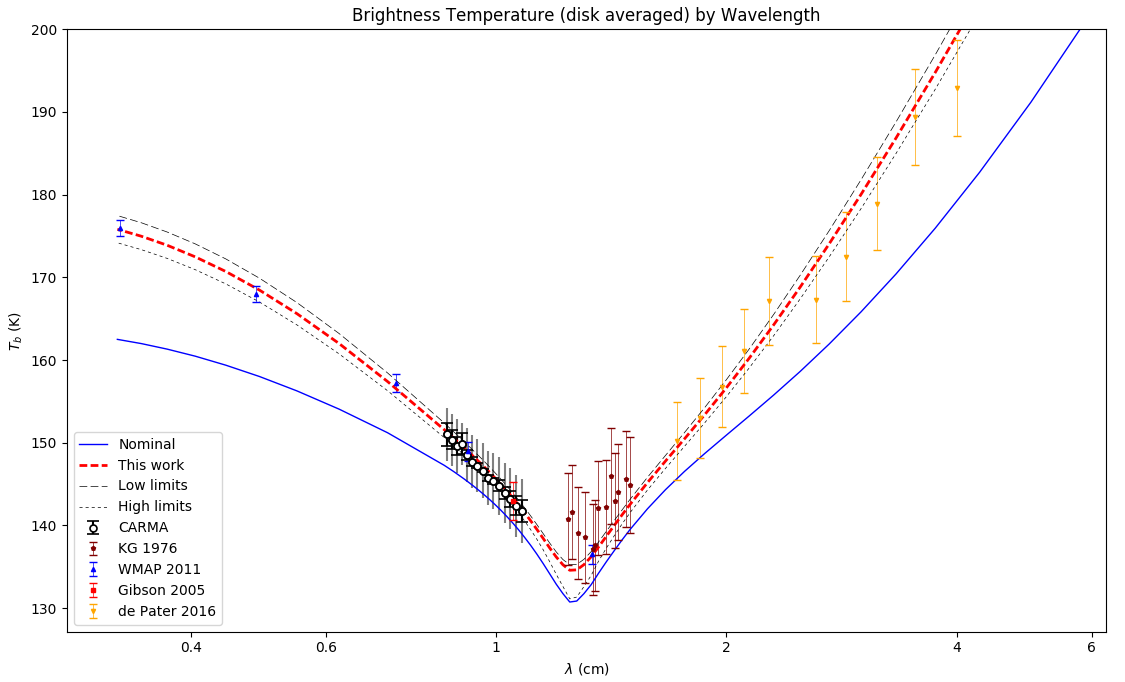
\includegraphics[width=\textwidth]{final_models_wl.png}
		\caption{\label{fig:emission_wl}CARMA measurements of disk-averaged brightness temperature together with extant measurements. Nominal model is included, as well as the model we suggest in this work, using parameters discussed in Section \ref{s:results}, and the global high- and low-abundance limits. The lower limit for high atmospheric abundance is, as discussed in the text, not stated in this work. CARMA measurements are shown with relative certainty at the capped error bars and absolute uncertainty at the larger, uncapped bars. Note the uniformity in absolute certainty and the frequency-dependent variation in relative uncertainty.}
	\end{figure}

	\begin{figure}
		\centering
		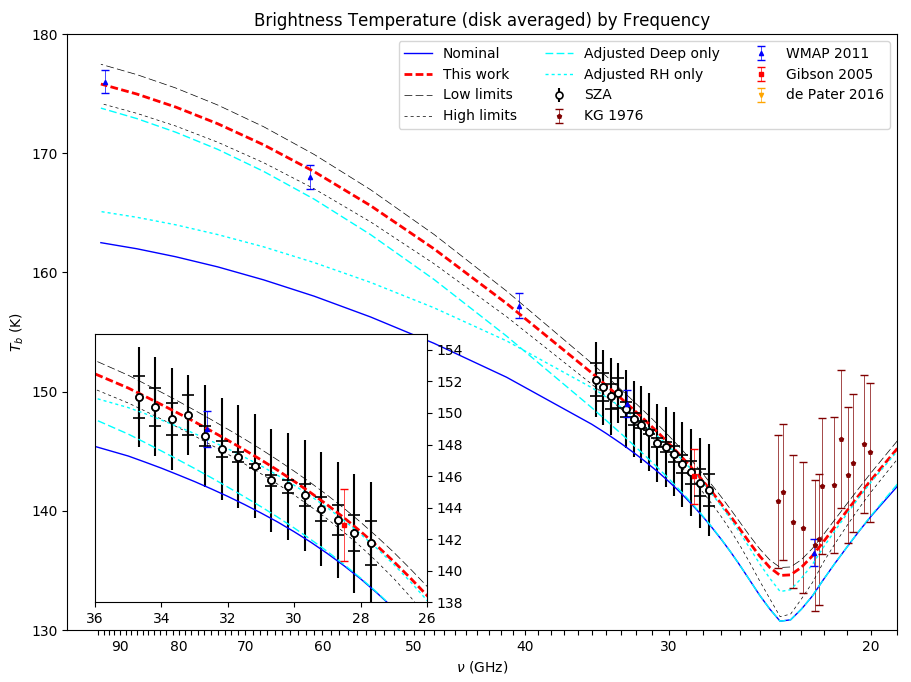
\includegraphics[width=\textwidth]{final_models_freq.png}
		\caption{\label{fig:emission_freq}Similar to Figure \ref{fig:emission_freq}, but restricted to a smaller spectral range and set against a frequency axis. Inset panel provides a clearer view of the CARMA points reduced in this work. We include two additional models, indicated by cyan lines, representing one-parameter deviations from the nominal model; in other words, we hold two parameters at 100\% of the nominal value and let the third take on the preferred value based on the $\chi^{2}$ fit so as to demonstrate the effects of the parameters as well as their general independence to each other. The effects of relative humidity and deep atmosphere abundance are shown by the two cyan lines. High atmosphere abundance is not shown here, but when decreased raises the temperature at the band center and accounts for the band center difference between the relative-humidity-only and preferred (red-dashed) models.}
	\end{figure}


\section{Conclusion}

	We began with 37 secondary calibration scans of Jupiter over the course of 5 months, made with CARMA at 15 different frequencies between 27-35 GHz.
	From there, we reduced this into 15 measurements of Jupiter's thermal brightness, limited to the case of the disk-averaged atmosphere.
	With these data, we filled in a $\sim 10$ GHz wide section of Jupiter's thermal emission profile, near an NH$_{3}$ absorption band.
	CARMA's strong spectral stability lends our data a strong certainty in slope, so we used this slope measurement as well as our absolute calibration, to some degree, and several surrounding data to better characterize the band shape.
	We modeled to this band shape by designing a model-comparison process around a radiative transfer code and found that, compared to the nominal abundance value, our characterization of the band shape suggests a globally lower abundance, to varying degrees at three distinct pressure regions in the atmosphere.
	Deep atmosphere abundance between $P < 8$ bar and the $P \sim 0.8$ bar condensation point is found to be $2.40\e{-4}$, bounded between $[2.26, 2.57] \e{-4}$.
	Relative humidity, within the NH$_{3}$ cloud layer where abundance follows the saturation curve, is found to be $56.5\%$, bounded between $[50\%, 63.5\%]$.
	Top atmosphere abundance, above the NH$_{3}$ cloud layer and past the departure from the saturation curve, is found to have an upper bound of $2.4\e{-7}$, but is indicated through two separate analysis methods to be closer to $2\e{-8}$.
	These results seem to echo the conclusion made in JG, especially that of subsaturation by a factor of 2.

	We hope that this measurement set will be useful in future explorations, as have WMAP, Gibson, and others been in ours.
	These results are of course limited to the case of the disk-averaged atmosphere, and we look forward to ongoing and future projects who will expand this research to the spatially resolved case.
	We look forward to the release of data from the Juno probe mission in particular; while its investigation will involve some spatial resolution, it may serve to confirm or correct our findings.

	CARMA's calibration is strong enough that we feel these reduced thermal measurements may be useful as calibration information for interferometers lacking short baselines.
	The measurements produced in this work are believed to encompass all flux from the disk, so they may be treated as ``single-dish'' flux measurements to give calibration context to interferometer scans.



\section{References}

\bibliographystyle{apj}
\bibliography{projectwriteup}


\end{document}